%    \begin{macrocode}
\documentclass[color,table,nolot,nolof]{fithesis3}
\usepackage[english]{babel}
\usepackage{hologo}
\usepackage{fancyvrb}
\usepackage{minted}
\usepackage{ltxcmds}
\usepackage{tabularx}
\usepackage[
  backend=biber,
  style=numeric,
  citestyle=numeric-comp,
  sorting=none,
  sortlocale=auto
]{biblatex}
\addbibresource{guide.bib}
\usepackage[os=win]{menukeys}
\makeatletter
\thesissetup{
  title=A fibeamer user guide for the \thesis@english@facultyName,
  TeXtitle=A \textit{fibeamer} user guide\medskip\\\Large for the
    \thesis@english@facultyName,
  type=bc,
  department=Department of Computer Graphics and Design,
  programme=Applied Informatics,
  field=Typesetting,
  titleEn=\thesis@title,
  departmentEn=\thesis@department,
  programmeEn=\thesis@programme,
  fieldEn=\thesis@field,
  author=Vít Novotný,
  advisor={Doc.\ RNDr.\ Petr Sojka, Ph.D.},
  assignment={},
  abstract={\textsf{Fibeamer} is a theme for the \textsf{beamer}
    \LaTeX{} document class and is intended to be used for the
    preparation of thesis defense presentations across the
    faculties of the \thesis@english@universityName. This document
    describes the installation of the \textsf{fibeamer} theme, its
    configuration, and its use.},
  keywords={thesis, typesetting, LaTeX},
  TeXkeywords={thesis, typesetting, \LaTeX{}},
  keywordsEn=\thesis@keywords,
  TeXkeywordsEn=\thesis@TeXkeywords,
  abstractEn=\thesis@abstract,
  faculty=\jobname,
  autoLayout=false}
\makeatother
\begin{document}
  \makeatletter\thesis@preamble\makeatother
  \chapter{Introduction}
  To use the \textsf{fibeamer} beamer theme, you can use an online
  \LaTeX{} editor, such as Overleaf%
  \footnote{Overleaf \textsf{fibeamer} templates are located at
  \url{http://www.overleaf.com/gallery/tagged/muni}.},
  which allows you to skip the installation described in Section
  \ref{sec:install} completely.
  
%<*fi>
  {\makeatletter\newcount\thguide@tl\expandafter\thguide@tl\the
  \year\if\month<7\advance\thguide@tl-1\fi\makeatother
  Another way to avoid installation is to use any public-access
  computer at the \makeatletter\thesis@english@facultyName
  \makeatother\ that runs Microsoft Windows. By running
  \begin{center}
    \makeatletter\menu[,]{Start,Programs,Document Tools,TeXLive%
    \the\thguide@tl\ namapovani na T}\makeatother
  \end{center} you can mount the faculty \TeX\ Live installation to
  drive \verb'T:\'. Consequently, you can either use the command
  line to run commands from the \TeX{} distribution by running
  \begin{center}
    \makeatletter\menu[,]{Start,Programs,Document Tools,TeXLive%
    \the\thguide@tl\ CMD}\makeatother
  \end{center}
  or you can use the graphical \TeX\ editor \TeX Works by running
  \begin{center}
    \makeatletter\menu[,]{Start,Programs,Document Tools,TeXWorks+%
    TeXLive\the\thguide@tl}\makeatother
  \end{center}}

  Yet another way to avoid installation is to either connect to the
  Linux server at \url{aisa.fi.muni.cz} over SSH, or use any
  public-access computer at the
  \makeatletter\thesis@english@facultyName\makeatother\ that runs
  Linux or Mac OS, and load the faculty \TeX\ Live installation by
  issuing the \texttt{module add texlive} command on the command
  line. If you choose this approach, you can also skip the entire
  Section \ref{sec:install}, although a certain degree of
  proficiency in working with a Unix operating system is required
  compared to the other methods.
%</fi>
  \makeatletter
    % This macro kerns an icon next to a word.
    \def\thguide@iconkern{\kern.2ex}
  \makeatother
%<*sci>
  \makeatletter
    % This macro typesets the URL of a math.muni server.
    \def\thguide@server#1{%
      \includegraphics[height=.5em]{resources/#1.pdf}%
      \thguide@iconkern\url{#1.math.muni.cz}}
  \makeatother
  Another way to avoid installation is to use the faculty \TeX\ Live
  installation by connecting to the Linux server at
  \makeatletter\thguide@server{yoda}\makeatother\ or
  \makeatletter\thguide@server{vader}\makeatother\ over SSH
  (through port 22222) or over the remote desktop
  protocol\footnote{
    For more information about connecting through the remote
    desktip protocol, see
    \url{http://www.math.muni.cz/aktuality/347-vzdaleny-pristup-yoda-vader.html}.}
  (through port 13556), or to use any public-access computer at the
  \makeatletter\thesis@english@facultyName\makeatother\ that runs
  Linux. If you choose this approach, you can also skip this entire
  section, although a certain degree of proficiency in working with
  a Unix operating system is required compared to the first method.
%</sci>
  
  \section{Installation}\label{sec:install}
  \subsection{Installing a \TeX{} distribution}
  If you decided not to use a public \TeX{} distribution, you will
  need to install one locally before proceeding further. A \TeX{}
  distribution contains tools and packages that are going to help
  you with preparing and typesetting your \LaTeX\ documents.

  The two major \TeX{} distributions that you can install are
  Mik\TeX\footnote{Mik\TeX\ can be acquired from
  \url{http://miktex.org/2.9/setup}.}, which can be used with the
  Microsoft Windows operating system, and \TeX\ Live\footnote{%
  \TeX\ Live can be acquired from
  \url{http://www.tug.org/texlive}.}, which can be installed on
  both Unix and Windows operating systems. The advantages of
  Mik\TeX\ include refined graphical user interface and the ability
  to install new packages on the fly.
  
  Along with Mik\TeX{}, you will also need to install a Perl
  interpreter, such as Strawberry Perl\footnote{Strawberry Perl can
  be downloaded from \url{http://strawberryperl.com/}.}. \TeX\ Live
  installs a Perl interpreter by default.

  \subsection{Installing packages}\label{sec:req-packages}
  In order to function properly, \textsf{fibeamer} needs the
  following packages packages to be installed in your \TeX\
  distribution: \textsf{ifthen}, \textsf{ifxetex},
  \textsf{ifluatex}, \textsf{lm}, \textsf{carlito}, \textsf{arev},
  \textsf{iwona}, \textsf{dejavu}, \textsf{setspace},
  \textsf{fontenc}, \textsf{fontspec}, \textsf{beamer},
  \textsf{fibeamer}.

  {\makeatletter %% A placeholder string macro
  \def\thguide@placeholder#1{$\langle$\textit{#1}$\rangle$} 
  If you performed a full installation of \TeX\ Live, you should
  already have all the required packages installed. If you are
  using a partial installation of \TeX\ Live, you can use the
  \texttt{tlmgr} command-line tool by executing \texttt{tlmgr
  install} \thguide@placeholder{pkgname}, where
  \thguide@placeholder{pkgname} is the name of the package you wish
  to install. In some cases, \TeX\ Live may assign a different name
  to a package. To find out the \TeX\ Live name of a package, open
  the
  \texttt{http://www.ctan.org/pkg/}\thguide@placeholder{pkgname}
  webpage in a web browser. It should contain the following text:
  \begin{center}
    Contained in \TeX\ Live as \thguide@placeholder{texlivename}
  \end{center}
  where \thguide@placeholder{texlivename} corresponds to the \TeX\
  Live name of the package. Use this name instead of
  \thguide@placeholder{pkgname} with \texttt{tlmgr}.
  Alternatively, you can download the packages manually from
  \texttt{http://www.ctan.org\discretionary{/}{/}{/}pkg/}%
  \thguide@placeholder{pkgname} and extract them into the
  \texttt{texmf/} directory located in your user home directory.
  Mind that the packages themselves may depend on other
  packages; if you are using a partial installation of \TeX\ Live,
  you will have to resolve these dependencies manually by
  inspecting the documentation of each package.

  If you use Mik\TeX\ and you enabled the \textit{over the air
  installation of packages} during the installation, Mik\TeX\ will
  automatically download all the required packages, when you first
  typeset a \textsf{fibeamer} document. If you didn't enable this
  feature, you will need to enter the Mik\TeX\ package manager by
  running
  \begin{center}
    \menu[,]{Start,MikTeX,MikTeX Package Manager (Admin)}
  \end{center}
  and download the packages manually through the user interface.
  In some cases, Mik\TeX\ may assign a different name to a 
  package. To find out the Mik\TeX\ name of a package, open the
  \texttt{http://www.ctan.org\discretionary{/}{/}{/}pkg/}%
  \thguide@placeholder{pkgname} webpage in a web browser,
  where \thguide@placeholder{pkgname} is the name of the
  package you wish to install. It should contain the following
  text:
  \begin{center}
    Contained in Mik\TeX\ as \thguide@placeholder{miktexname}
  \end{center}
  where \thguide@placeholder{miktexname} corresponds to the
  Mik\TeX\ name of the package. If you still can't find the
  package, try synchronizing the package database by selecting
  \begin{center}
    \menu[,]{Repository,Synchronize}
  \end{center}
  from the menu bar of the Mik\TeX\ package manager. Mind that the
  packages themselves may depend on other packages; if you disabled
  the over the air installation of packages, you will have to
  resolve these dependencies manually by inspecting the
  documentation of each package.}

  If you wish to use a newer version of \textsf{fibeamer} than the
  one that is available in your \TeX\ distribution, you should
  download a file named \texttt{fibeamer.tds.zip} containing the
  version of the package you wish to use and place it in a root
  directory that is recognized by your \TeX\ distribution. In
  \TeX\ Live\footnote{For more information about the \TeX\ Live root
  directories, see
  \url{http://www.tug.org/texlive/doc/texlive-en/texlive-en.html\#x1-110002.3},
  Chapter 2.3.}, one of such directories is the \texttt{texmf/}
  folder in your user home directory. In Mik\TeX\footnote{
  For more information about the \TeX\ Live root
  directories, see 
  \url{http://docs.miktex.org/manual/localadditions.html}.},
  the list of recognized root directories can be gleaned by
  running
  \begin{center}
    \menu[,]{Start,MikTeX,MikTeX Options (Admin),Roots}
  \end{center}

  \section{Picking a \TeX\ engine}
  There are several programs, called \TeX\ engines, that you can
  use to typeset \textsf{fibeamer} \LaTeX{} source files into
  displayable PDF documents. The ones we will discuss are
  \hologo{pdfTeX} and \Hologo{LuaTeX}.
  
  \Hologo{pdfTeX} is the more conservative choice and most \TeX\
  editors use \hologo{pdfTeX} as the default \TeX\ engine. The main
  advantage \Hologo{LuaTeX} over \hologo{pdfTeX} for a
  \textsf{fibeamer} user is the ability to use standard OpenType
  and TrueType fonts installed on your system, whereas
  \hologo{pdfTeX} is confined to the fonts installed in your \TeX\
  distribution.
  
  If the ability to use arbitrary fonts within your documents
  interests you, Chapter 3 of the \textsf{fontspec} package
  manual\footnote{The \textsf{fontspec} package manual is available
  at \url{http://mirrors.ctan.org/macros/latex/contrib/fontspec/fontspec.pdf}.}
  should provide you with the relevant information. If you are
  only going to use the fonts present in the \TeX{} distribution or
  if you do not intend to change the preset \textsf{fibeamer}
  fonts at all, you can safely use \hologo{pdfTeX}, which is
  currently also considerably faster than \Hologo{LuaTeX}.

  \section{Creating and typesetting a \textsf{fibeamer} document}
  Before using the \textsf{fibeamer} theme, it is useful to be
  familiar with the \LaTeX{} typesetting system. A good way to get
  started is to read one of the introductory texts in English
  \cite{veryshortlatex,shortlatex,longlatex,latex} or in Czech
  \cite{rybicka03,satrapa11}. Taking one of the \textit{FI:PB029},
  \textit{PřF:M5751}, or \textit{FF:PLIN028} courses taught at
  the \makeatletter\thesis@english@universityName\makeatother\ is
  also helpful.

  To become familiar with \textsf{fibeamer}, you are encouraged to
  inspect the example \textsf{fibeamer} documents named
  \makeatletter
  \texttt{\thesis@university-\thesis@faculty-pdflatex.pdf} and
  \texttt{\thesis@university-\thesis@faculty-lualatex.pdf} as well
  as their \LaTeX{} source files that are named
  \texttt{\thesis@university-\thesis@faculty-pdflatex.tex} and
  \texttt{\thesis@university-\thesis@faculty-lualatex.tex} that are
  distributed along with the package inside the \texttt{example/}
  directory\footnote{The example \textsf{fibeamer} documents are
  also available online at
  \url{https://www.ctan.org/tex-archive/macros/latex/contrib/beamer-contrib/fibeamer/example/mu}.}.
  By modifying and by typesetting these \LaTeX{} source files using
  either the \hologo{pdfTeX} or the \Hologo{LuaTeX} engine, you can
  quickly gain a working knowledge of \LaTeX{} and use these source
  files as the basis for your thesis. To typeset the example
  documents, you need to download the \texttt{resources/} directory
  as well, as it contains vector images used in the examples.
  
  If you are using an online editor, such as Overleaf
  \footnote{Overleaf \textsf{fibeamer} templates are located at
  \url{http://www.overleaf.com/gallery/tagged/muni}.}, \LaTeX{}
  source files will be typeset automatically, as you edit them. The
  \TeX{} engine can be selected inside the
  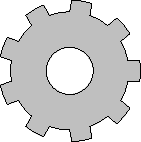
\includegraphics[height=1.3ex]{resources/cog.pdf}\makeatletter
  \thguide@iconkern\makeatother project settings.

  If you are using a graphical \TeX{} editor, such as \TeX
  works\footnote{\TeX works can be downloaded from
  \url{http://www.tug.org/texworks/}.}, you can typeset a \LaTeX{}
  source file by opening the source file from within the editor and
  running either the \hologo{pdfLaTeX} or \Hologo{LuaLaTeX}
  (depending on your choice of \TeX\ engine) command from the task
  bar. The command needs to be executed at least twice.

  If you are using the command line, you can typeset \LaTeX{}
  source files by running either \texttt{pdflatex
  \textit{name.tex}} or \texttt{lualatex
  \textit{name.tex}} (depending on your choice of \TeX\
  engine), where \texttt{\textit{name.tex}} corresponds to the name
  of a \LaTeX\ source file. In the case of the two aforementioned
  example files, the corresponding commands would be:
  \begin{center}\makeatletter
  \texttt{pdflatex \thesis@university-\thesis@faculty-pdflatex.tex}
\\\texttt{lualatex \thesis@university-\thesis@faculty-lualatex.tex}
  \makeatother\end{center}
  The command needs to be executed from within the directory, where
  the \LaTeX\ source file is located. In Windows, the command line
  can be opened in a directory by holding down the \keys{Shift} key
  and by clicking the right mouse button while hovering the cursor
  over a directory. Select the \menu{Open Command Window Here}
  option in the context menu that opens shortly afterwards.  The
  command also needs to be executed at least twice.

  Beside Overleaf and \TeX works, any text editor can be used to
  modify \LaTeX{} source files.

  \chapter{Configuration}
  A \textsf{fibeamer} \LaTeX{} source file should begin as follows:
  \begin{minted}{latex}
\documentclass{beamer}
\usetheme[option1, option2, ..., optionN]{fibeamer}
  \end{minted}
  The following list summarizes the options that are recognized by
  the \textsf{fibeamer} theme and their meaning. Options that are
  enabled by default are \textit{set in italics}.

  {\makeatletter
  % This macro formats a default class option.
  \def\thguide@default{\itshape}
  % This macro formats a class option.
  \let\thguide@itemfmt\textbf
  \begin{description}
    \item[faculty=$\langle${name}$\rangle$]
      This option changes the color theme based on the selected
      faculty. To choose the color theme of the
      \thesis@english@facultyName, use
      {\thguide@itemfmt\thesis@faculty} as the
      $\langle$name$\rangle$.
    \item[\thguide@default fonts]
      This option sets up the combination of the font families of
      Carlito, Arev, Iwona, Dsfont, and DejaVu for the typesetting
      of text and mathematics.
    \item[nofonts]
      This option prevents \textsf{fibeamer} from setting up the
      fonts. The user must set the fonts manually in the preamble
      of the document.
%<*fi>

      The \thesis@english@facultyName\ has licensed the Comenia
      font family. If you wish to use it in your thesis, you should
      contact Doc.\ RNDr.\ Petr Sojka, Ph.D.
      
      If you are typesetting your thesis on a public-access
      computer at the \thesis@english@facultyName\ or on the
      \url{aisa.fi.muni.cz} Linux server, you can use the
      commercial Math Time mathematical font family,
%</fi>
%<*sci>

      If you are typesetting your thesis on a public-access
      computer at the \thesis@english@facultyName\ that runs Linux
      or on either the \thguide@server{yoda} or
      \thguide@server{vader} Linux server, you can also use the
      commercial Math Time mathematical font family,
%</sci>
%<*sci,fi> 
      which goes well with the \TeX\ Gyre Termes text font family.
      To use Math Time and \TeX\ Gyre Termes within your thesis,
      the preamble of your document should look as follows:
      \begin{minted}{latex}
\documentclass{beamer}
\usetheme[nofonts, ...]{fibeamer}
\usepackage[utf8]{inputenc}
\usepackage[T1]{fontenc}
\usepackage{tgtermes}
\usepackage{mathtime}
%% Here goes the rest of the document.
      \end{minted}
%</sci,fi>
    \item[\thguide@default microtype]
      This option sets up microtypographic extensions\footnote{
        For more information about the \TeX\ engine
        microtypographic extensions, see
        \url{http://mirrors.ctan.org/macros/latex/contrib/microtype/microtype.pdf}.
      }, which results in visually more pleasing paragraphs of
      text.
    \item[nomicrotype]
      This option prevents \textsf{fibeamer} from setting up
      microtypographic extensions. 
  \end{description}
  The complete list of the package options can be found in Section
  2 of the technical documentation of the \textsf{fibeamer}
  class \cite{novotny15}.}

  \makeatletter\thesis@postamble\makeatother
  \tolerance=300\emergencystretch=1em
  \printbibliography[heading=bibintoc]
\end{document}
%    \end{macrocode}
